% includemthe figures path relative to the master file
\graphicspath{ {./content/other/figures/} }

\section{other}
\label{sec:other}  % \label{} allows reference to this section

This section is used testing that the packages perform as expected regardless of the template in hand.

\subsection{Citations}
\label{sec:other:citations}
% This file is an addaptation of the biblatex citation example that can be
% found at:
%   http://www.ctan.org/tex-archive/macros/latex/contrib/biblatex/doc/examples/
%
% The example uses the database biblatex-examples.bib.
% \addbibresource{biblatex-examples.bib}
%
% Some generic settings.
\newcommand{\cmd}[1]{\texttt{\textbackslash #1}}
\setlength{\parindent}{0pt}

This section adapts this
\href{http://www.ctan.org/tex-archive/macros/latex/contrib/biblatex/doc/examples/01-introduction.tex}{example}
in order to illustrate the usage of the \emph{biblatex} package with a biber backend.
Dudring the development of the document, the bibligraphic style is recomended to be set up as \textbf{draf}
(see this \href{http://mirrors.ircam.fr/pub/CTAN/macros/latex/contrib/biblatex/doc/examples/81-style-draft.pdf}{example}).
The full \emph{biblatex} documentation can be found \href{http://www.ctan.org/pkg/biblatex}{here}.

\begin{description}
  \item [Style-dependent] \cmd{cite} \cmd{parencite} \cmd{footcite} \cmd{textcite}
  \item [Sytle-independent] \cmd{autocite}
  \item [Text ingegrated] \cmd{citeauthor} \cmd{citetitle} \cmd{citetitle*} \cmd{citeyear}
  \item [Special] \cmd{nocite} \cmd{fullcite} \cmd{footfullcite}
\end{description}

\subsubsection*{The \cmd{cite} command}

Prints a bare citation without parentheses, that can be called
as it is, \cmd{cite\{key\}} producing \cite{companion};
~$\cdot$~
indicating a reference page (or range) \cmd{cite[59]\{key\}} producing \cite[59]{companion};
~$\cdot$~
with a note \cmd{cite[see][]\{companion\}} producing \cite[see][]{companion};
~$\cdot$~
or both \cmd{cite[see][59--63]\{companion\}} \cite[see][59--63]{companion}.

\subsubsection*{The \cmd{parencite} command}

This command, which is intended for in-text citations,
encloses the citation in parentheses. Note that the 'numeric' and
'alphabetic' styles use square brackets instead.
Like before it can be called as it is, \cmd{parencite\{key\}} producing \parencite{companion};
~$\cdot$~
indicating a reference page (or range) \cmd{parencite[59]\{key\}} producing \parencite[59]{companion};
~$\cdot$~
with a note \cmd{parencite[see][]\{companion\}} producing \parencite[see][]{companion};
~$\cdot$~
or both \cmd{parencite[see][59--63]\{companion\}} \parencite[see][59--63]{companion}.

\subsubsection*{The \cmd{footcite} command}

is similar to \cmd{parencite}, except that the
citation is given in a footnote.
It can be called as it is, \cmd{footcite\{key\}} producing \footcite{companion};
~$\cdot$~
indicating a reference page (or range) \cmd{footcite[59]\{key\}} producing \footcite[59]{companion};
~$\cdot$~
with a note \cmd{footcite[see][]\{companion\}} producing \footcite[see][]{companion};
~$\cdot$~
or both \cmd{footcite[see][59--63]\{companion\}} \footcite[see][59--63]{companion}.

\subsubsection*{The \cmd{textcite} command}

is intended for citations integrated in the
flow of text, replacing the subject of the sentence.

\textcite{companion} show that this is just filler text called as
\cmd{texcite\{key\}}, which can also be called with a parameter
\cmd{textcite[59]\{key\}} to produce \textcite[59]{companion} showing
that this is just filler text.

With \cmd{textcite}, the first optional argument is of limited use
only, since you could simply place the prenote in front of the
citation. It is still supported for the sake of consistency.

\textcite[see][]{companion} show that this is just filler text
produced by \cmd{textcite[see][]\{companion\}}
while \cmd{textcite[see][59--63]\{companion\}} produces
\textcite[see][59--63]{companion} plus some text filler.


\subsubsection*{The \cmd{autocite} command}

The point of the \cmd{autocite} command is that it automatically adapts
to the predominant citation format (inline or footnote) normally
used with the selected citation style. It should be used at the
end of the sentence and usually works like \cmd{parencite} or
\cmd{footcite}, depending on the citation style and the setting of the
'autocite' package option. With the author-year style used in this
example, it works like \cmd{parencite}:

This is just filler text \autocite{companion}.

\subsubsection*{Text commands}

There are a few predefined commands for bibliographic data which
is frequently used in the flow of text. 
Like \cmd{citeauthor} to recall the author, \cmd{citetitle} for
the short-title when available, \cmd{citetitle*} for the full title, 
or \cmd{citeyear} to retrieve the year.

\citetitle*{companion} by \citeauthor{companion} was
published in \citeyear{companion} has the following short-title:
\citetitle{companion}.

Note that biblatex also grants access to all lists and fields at a lower level,
see documentation.




%Here is the text of your introduction using some \ac{a}, referencing some \cref{eq:simple_equation} and citing \cite{Xbook_full}.%\citeauthor{Xbook}.
%\lipsum[2]
%
%\begin{equation}
%    \label{eq:simple_equation}
%    \alpha = \sqrt{ \beta }
%\end{equation}
%
%\lipsum[3]
%
%\begin{figure}
%    \centering
%    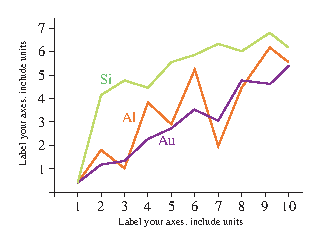
\includegraphics[width=3.0in]{fig_1}
%    \caption{Simulation Results}
%    \label{fid:simulationfigure}
%\end{figure}
%
%
%Write your subsection text here\,\cite{Xarticle}.

% \subsection{Subsection testing \emph{acro}}
% \label{sec:intro:acro}
% Example showing how plurals are easily handeled:
% first time: \ac{a} \\
% second time: \ac{a} \\
% short: \acs{a} \\
% alternative: \aca{a} \\
% first again: \acf{a} \\
% long: \acl{a} \\
% short plural: \acsp{a} \\
% long plural: \aclp{a} \\

% Here is an example of using the package taken from \cite{acro_sOverflow_url}.
% The example uses nested declarations and calls the acronyms using macros.

% \subsubsection*{nested acronyms example 1}

% \Ac{dna} is a very important molecule.  The virus xyz contains \dsdna.  Apart
% from that, \dna exists in almost all cells of the body. In most cases it is
% \dsdna.

% \subsubsection*{nested acronyms example 2}
% \acresetall

% The virus xyz contains \dsdna.  \Ac{dna} is a very important molecule.  Apart
% from that, \dna exists in almost all cells of the body. In most cases it is
% \dsdna.

% Some stuff that emac's colegues use
%%% Local Variables:
%%% mode: late
%%% TeX-master: "../../master.tex"
%%% End: \section{other}

